\documentclass[../../main.tex]{subfiles}

\begin{document}

\section{Programozás II}

\begin{fulltheorem}
  Fuzzy rendszerek.
\end{fulltheorem}


\paragraph{Fuzzy szabályok} A fuzzy szabályok alapjai:
\begin{itemize}
  \item \texttt{HA $x = A$, AKKOR $y = B$}
        \begin{itemize}
          \item $A$ -- a szabály accendense
          \item $B$ -- a szabály konzekvense
        \end{itemize}
  \item Pl.: \texttt{HA} a forgalom erős északi irányban,
        \texttt{AKKOR} a lámpa legyen hosszabb ideig zöld.
\end{itemize}

\begin{figure}[htb]
  \centering
  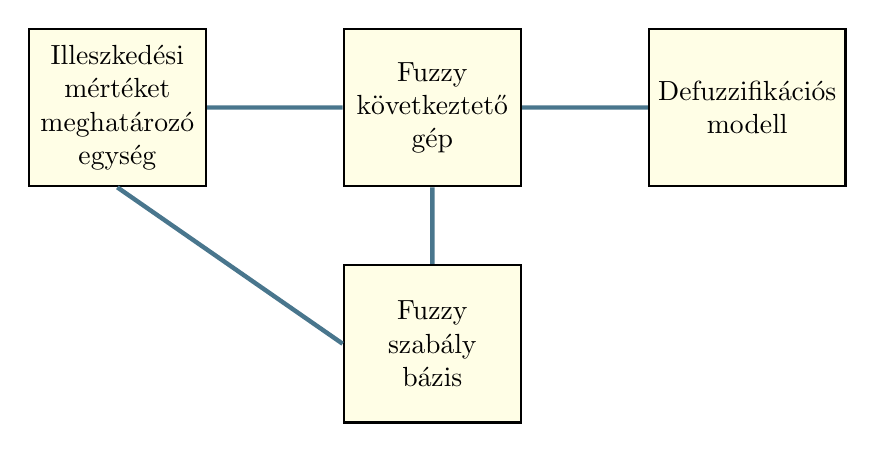
\begin{tikzpicture}[
      thick,
      box/.style={
          rectangle,
          align=center,
          draw=black, fill=yellow!10,
          minimum height=2cm, minimum width=2.25cm,
        }
    ]
    \node[box] (l) at (-4,0) {Illeszkedési\\mértéket\\meghatározó\\egység};
    \node[box] (t) at (0,0) {Fuzzy\\következtető\\gép};
    \node[box] (r) at (4,0) {Defuzzifikációs\\modell};
    \node[box] (b) at (0,-3) {Fuzzy\\szabály\\bázis};

    \draw[cyan!50!black, ultra thick]
    (l) -- (t)
    (t) -- (r)
    (t) -- (b)
    (l.270) -- (b.180)
    ;
  \end{tikzpicture}
  \caption{A fuzzy rendszer általános sémája}
  \label{fig:fuzzy-scheme}
\end{figure}

\paragraph{Példa} A motor fuzzy szabályozása
\begin{itemize}
  \item \texttt{HA} a hőmérséklet \textit{HIDEG},
        \texttt{AKKOR} a motor sebesség \textit{ALACSONY}.
  \item \texttt{HA} a hőmérséklet \textit{MELEG},
        \texttt{AKKOR} a motor sebesség \textit{KÖZEPES}.
  \item \texttt{HA} a hőmérséklet \textit{FORRÓ},
        \texttt{AKKOR} a motor sebesség \textit{MAGAS}.
\end{itemize}

\paragraph{Példa} Az emberek magasságát leíró fuzzy halmazok.
\begin{itemize}
  \item A halmazok részben átfedésben vannak.
  \item Egy ember több halmazba is beletartozhat.
\end{itemize}
\begin{figure}[htb]
  \centering
  \includegraphics{../../static/tex/build/fuzzy-height.pdf}
  \caption{Az emberek magasságát leíró fuzzy halmazok}
  \label{fig:fuzzy-height}
\end{figure}
\begin{align*}
  \core {\color{cyan!50!black}K}     & = [170; 180]                   \\
  \supp {\color{cyan!50!black}K}     & = [160; 190]                   \\
  {\color{cyan!50!black}K}_{\alpha}  & = [160+10\alpha; 190-10\alpha] \\
  {\color{cyan!50!black}K}_{\alpha+} & = (160+10\alpha; 190-10\alpha) \\
  h(\color{cyan!50!black}K)          & = 1                            \\
\end{align*}

\end{document}
